\chapter{Instrukcja obsługi aplikacji}
Wygląd interfejsu użytkownika aplikacja w finalnej postaci różni się w kilku kwestiach od zaprojektowanych wcześniej makiet. Zmianie uległo ułożenie elementów menu głównego, dodano nowe przyciski: "Księga akordów" i "X". Dodano też dwa nowe widoki, których nie umieszczono na początkowych makietach: diagram akordów, zapisane akordy. Do obydwu z tych widoków można przejść jedynie z widoku księgi akordów, ponieważ stanowią one jego uzupełnienie. Dalsze zmiany omówiono przy okazji przedstawienia sposobu działania aplikacji. Każdy z widoków głównych, poza widokiem menu, zawiera przycisk ze znakiem "?", po naciśnięciu którego wyświetlona zostanie pomoc kontekstowa. \\[-10pt]

Po uruchomieniu aplikacji \emph{Guitarrr} na ekranie pojawi się menu główne z 6 przyciskami (rys~\ref{fig:Menu}). Naciśnięcie któregoś z nich skutkuje przeniesieniem do odpowiedniego widoku:
\begin{itemize}
    \item Metronom -- przenosi do widoku metronomu.
    \item Akordy gitarowe -- przenosi  do widoku księgi akordów.
    \item Stroik -- przenosi  do widoku stroika.
    \item Trening słuchu -- przenosi  do widoku treningu słuchu.
    \item Koło kwintowe -- przenosi do widoku koła kwintowego.
    \item X -- po jego naciśnięciu aplikacja zostanie wyłączona.
\end{itemize}
\begin{figure}[htb]
	\centering
	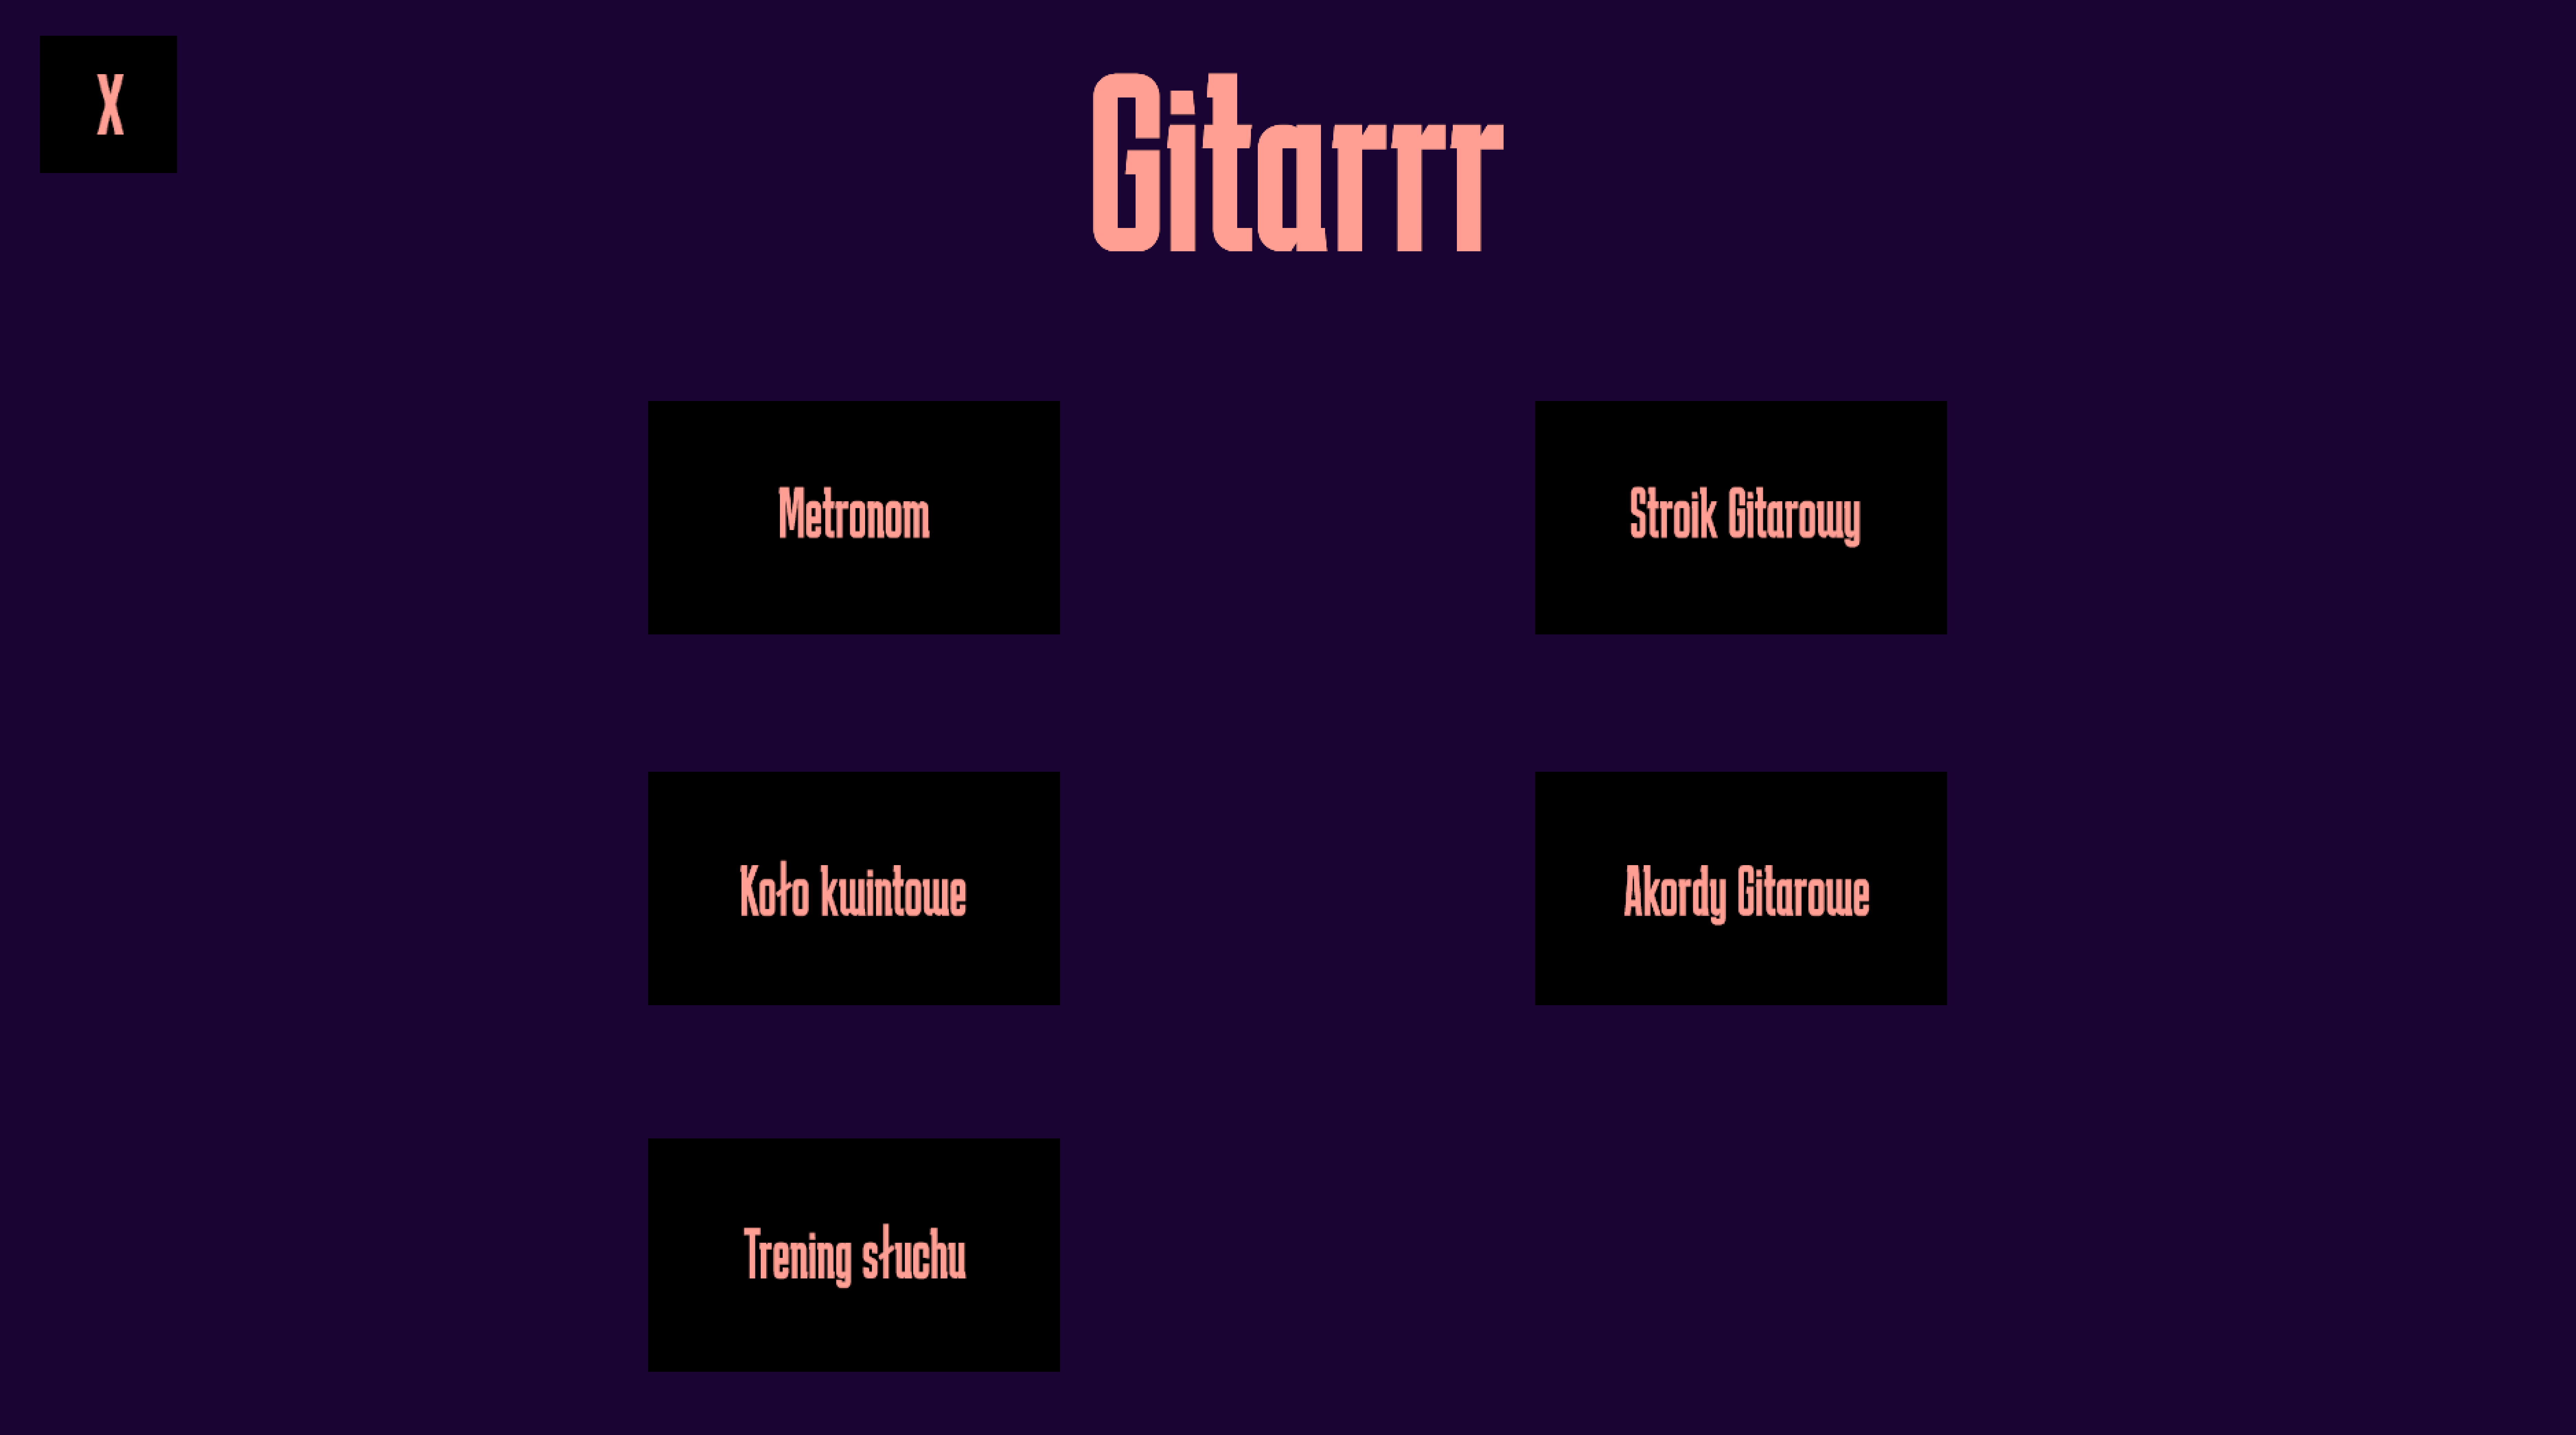
\includegraphics[width=.7\linewidth]{rysB/MenuG}
	\caption{Widok menu głównego} \label{fig:Menu}
\end{figure}

\paragraph{Metronom}
Porównując obecny widok metronomu z pierwotną makietą można zauważyć zmianę w elementach graficznych odpowiedzialnych za wybijanie taktów. Dodano indykator BPM i przyciski odpowiedzialne za jego zmianę oraz zmianę tempa i uruchomienie metronomu.

Korzystając z metronomu (rys.~\ref{fig:Metronom}), użytkownik ma dostęp do 2 przycisków odpowiedzialnych za zmianę liczby taktów (początkowo ustawione na 2) oraz 2 przyciski odpowiedzialne za zmianę liczby BPM (początkowo ustawione na 60). Aby dodać takt, należy nacisnąć przycisk z napisem "Dodaj takt", natomiast aby odjąć takt, użytkownik winien nacisnąć przycisk "Odejmij takt". Przycisk "+" służy do zwiększenia liczby BPM, natomiast "-" do ich zmniejszenia. Jeżeli użytkownik chciałby rozpocząć trening, należy nacisnąć przycisk "Start".

\begin{figure}[htb]
	\centering
	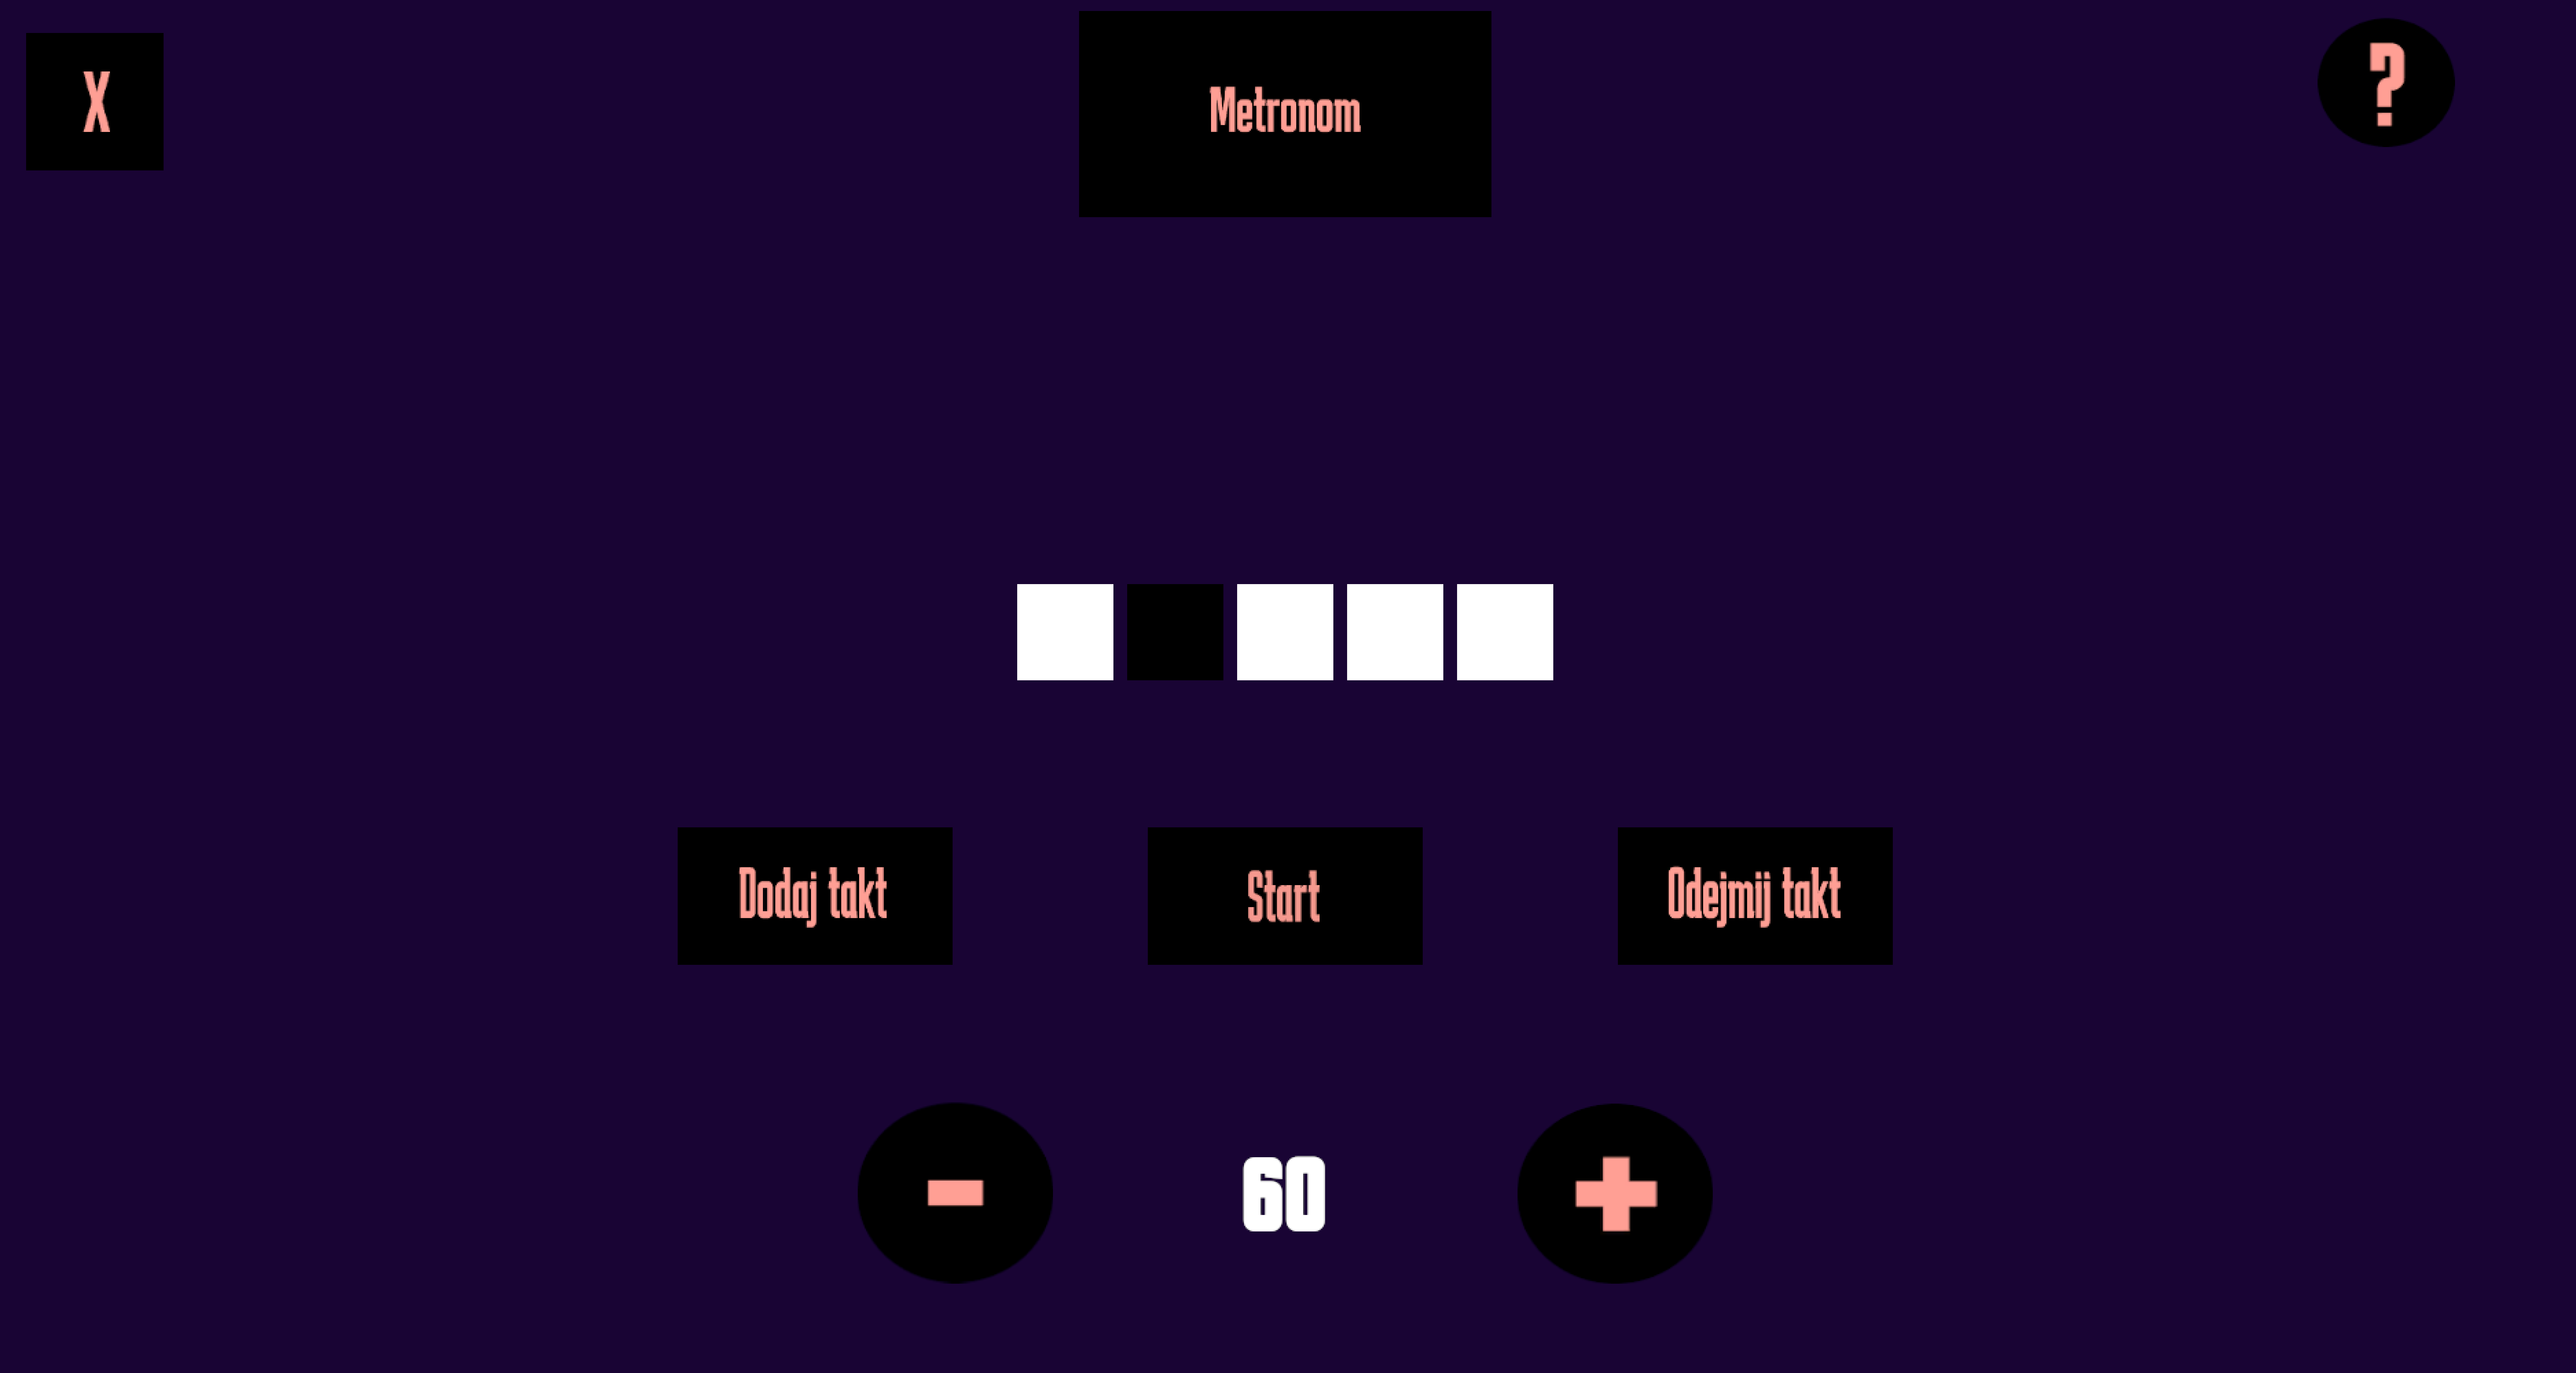
\includegraphics[width=.6\linewidth]{rysB/METRO.png}
	\caption{Widok metronomu} \label{fig:Metronom}
\end{figure}

% DONE: dołożyć widok metronomu

\paragraph{Księga akordów}
 Względem pierwotnej makiety uzupełniono ten widok o~przycisk informacji kontekstowej, przycisk wyjścia i przyciski przenoszące do widoków "diagramu akordów" i "zapisanych akordów" (rys.~\ref{fig:Ksiega_Zapisane}).
\begin{figure}[htb]
    \centering
		\begin{tabular}{l}
		a)  \\
		\vtop{\vskip-2ex\hbox{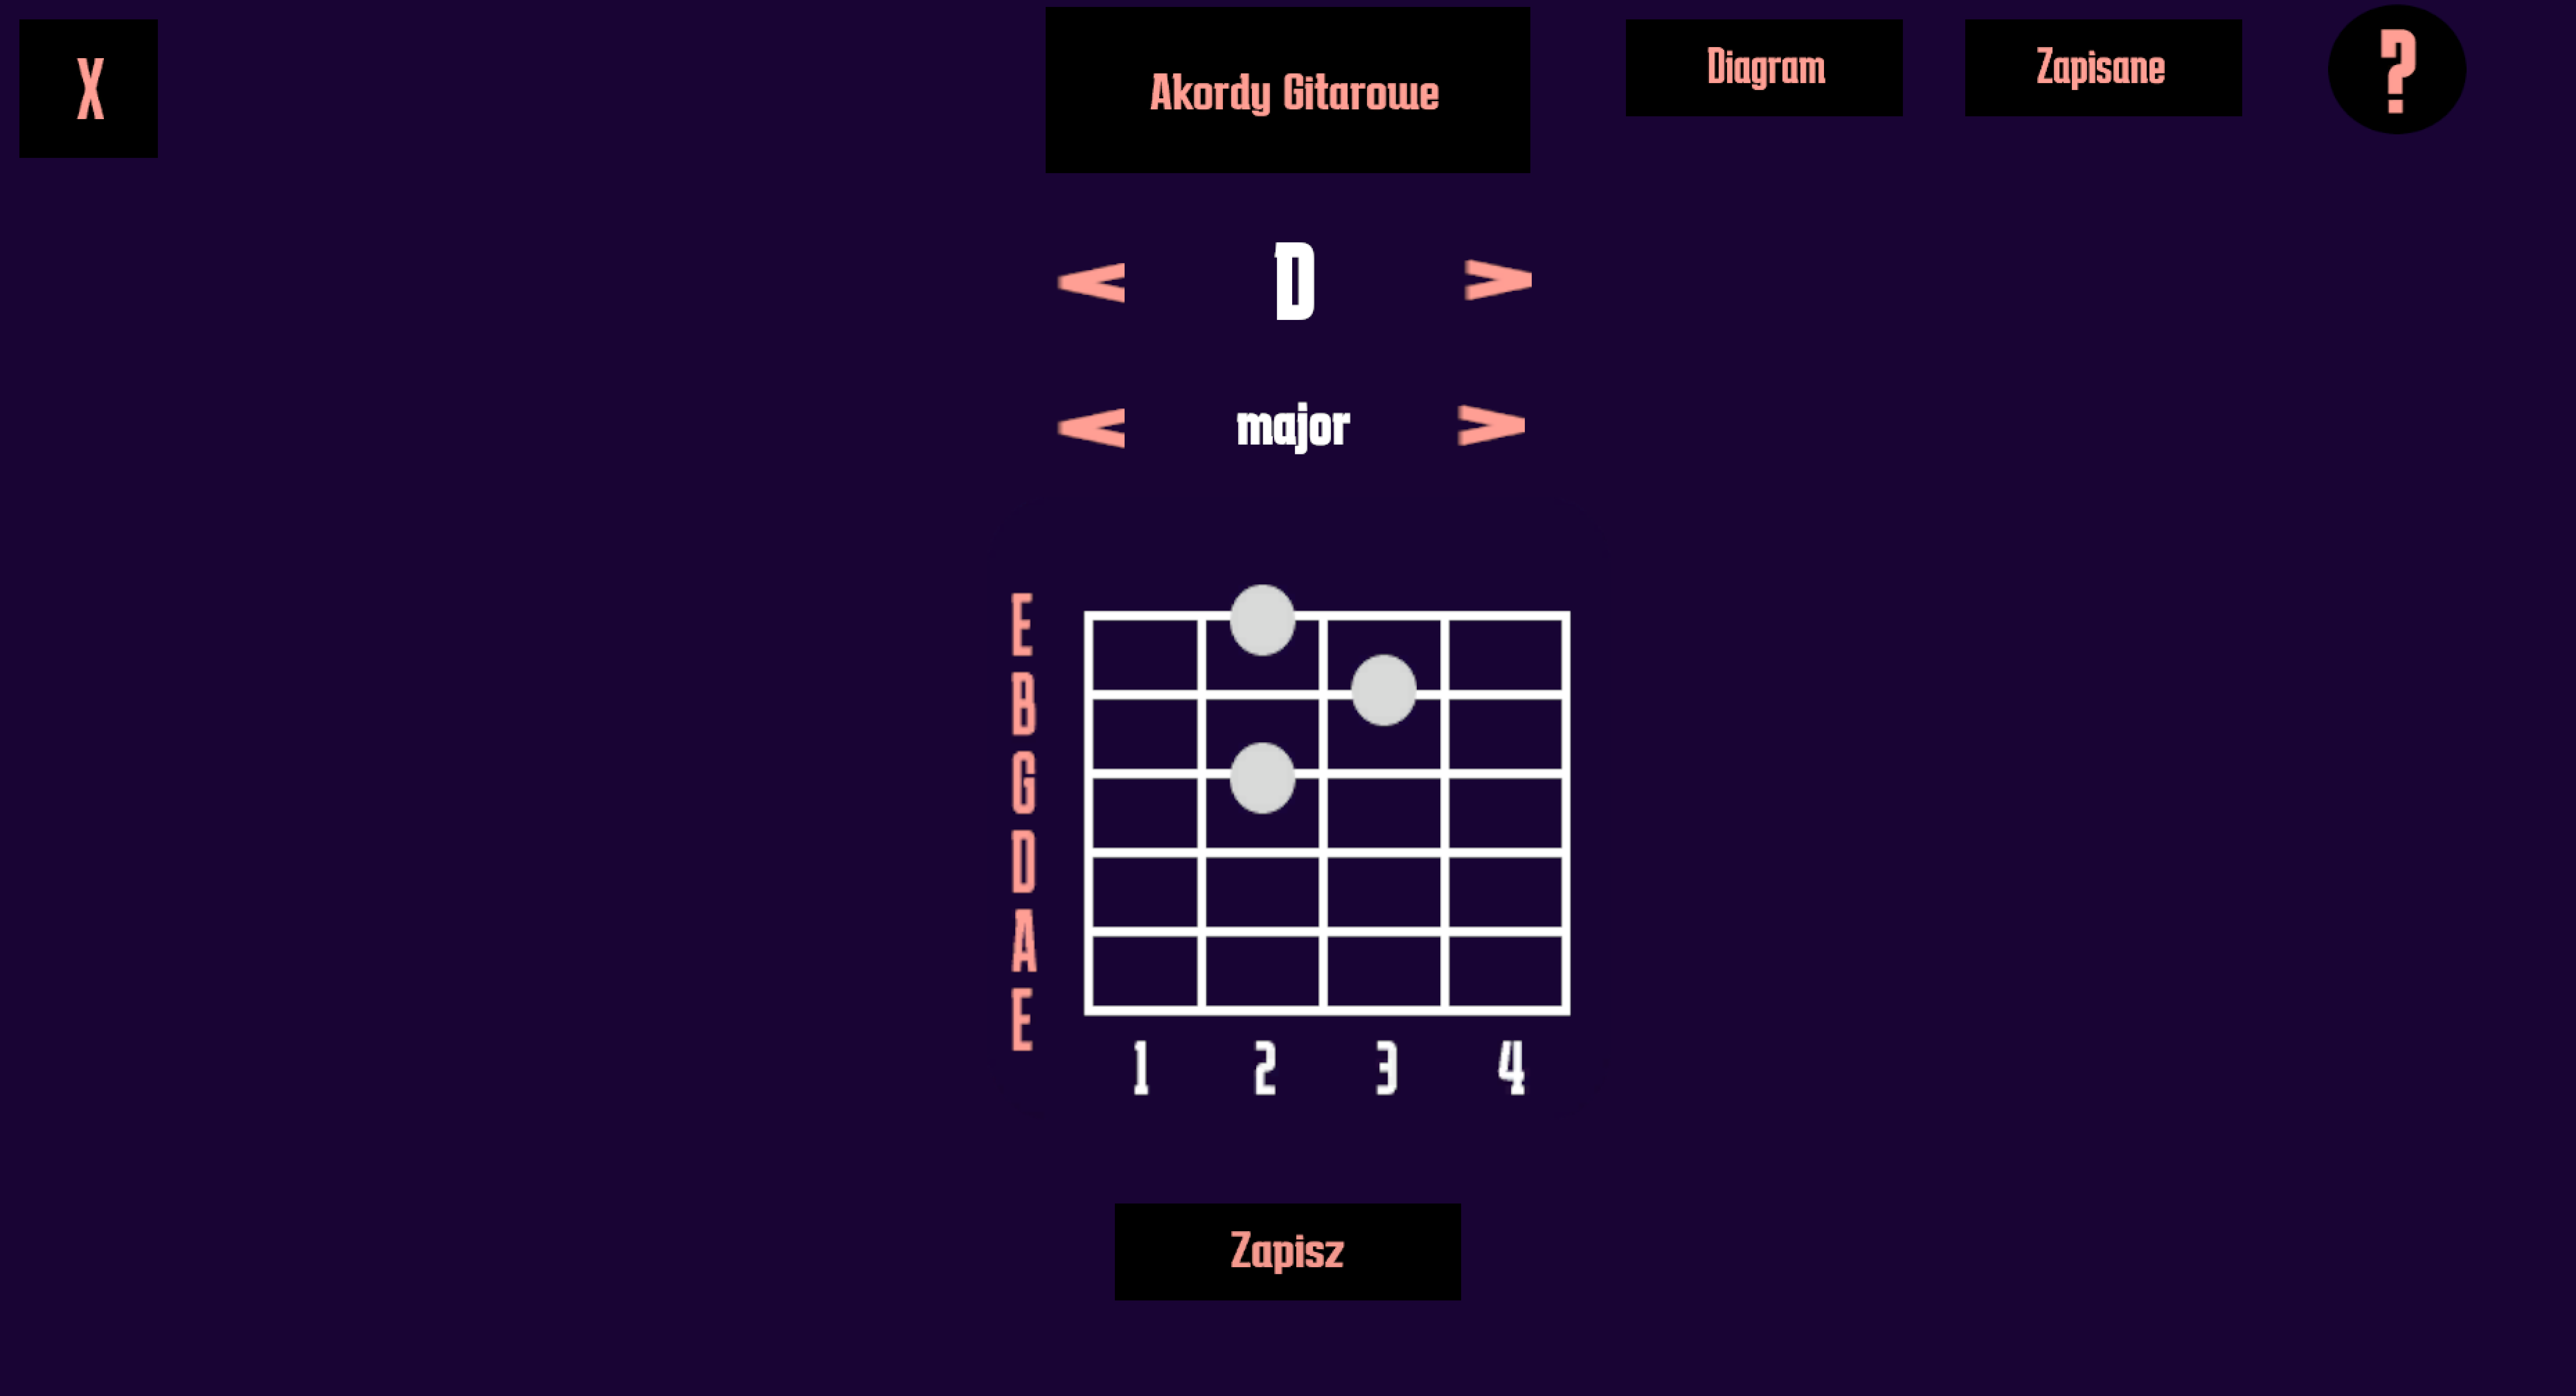
\includegraphics[width=0.6\linewidth]{rysB/Akordy}}} \\ 
		b) \\
		\vtop{\vskip-2ex\hbox{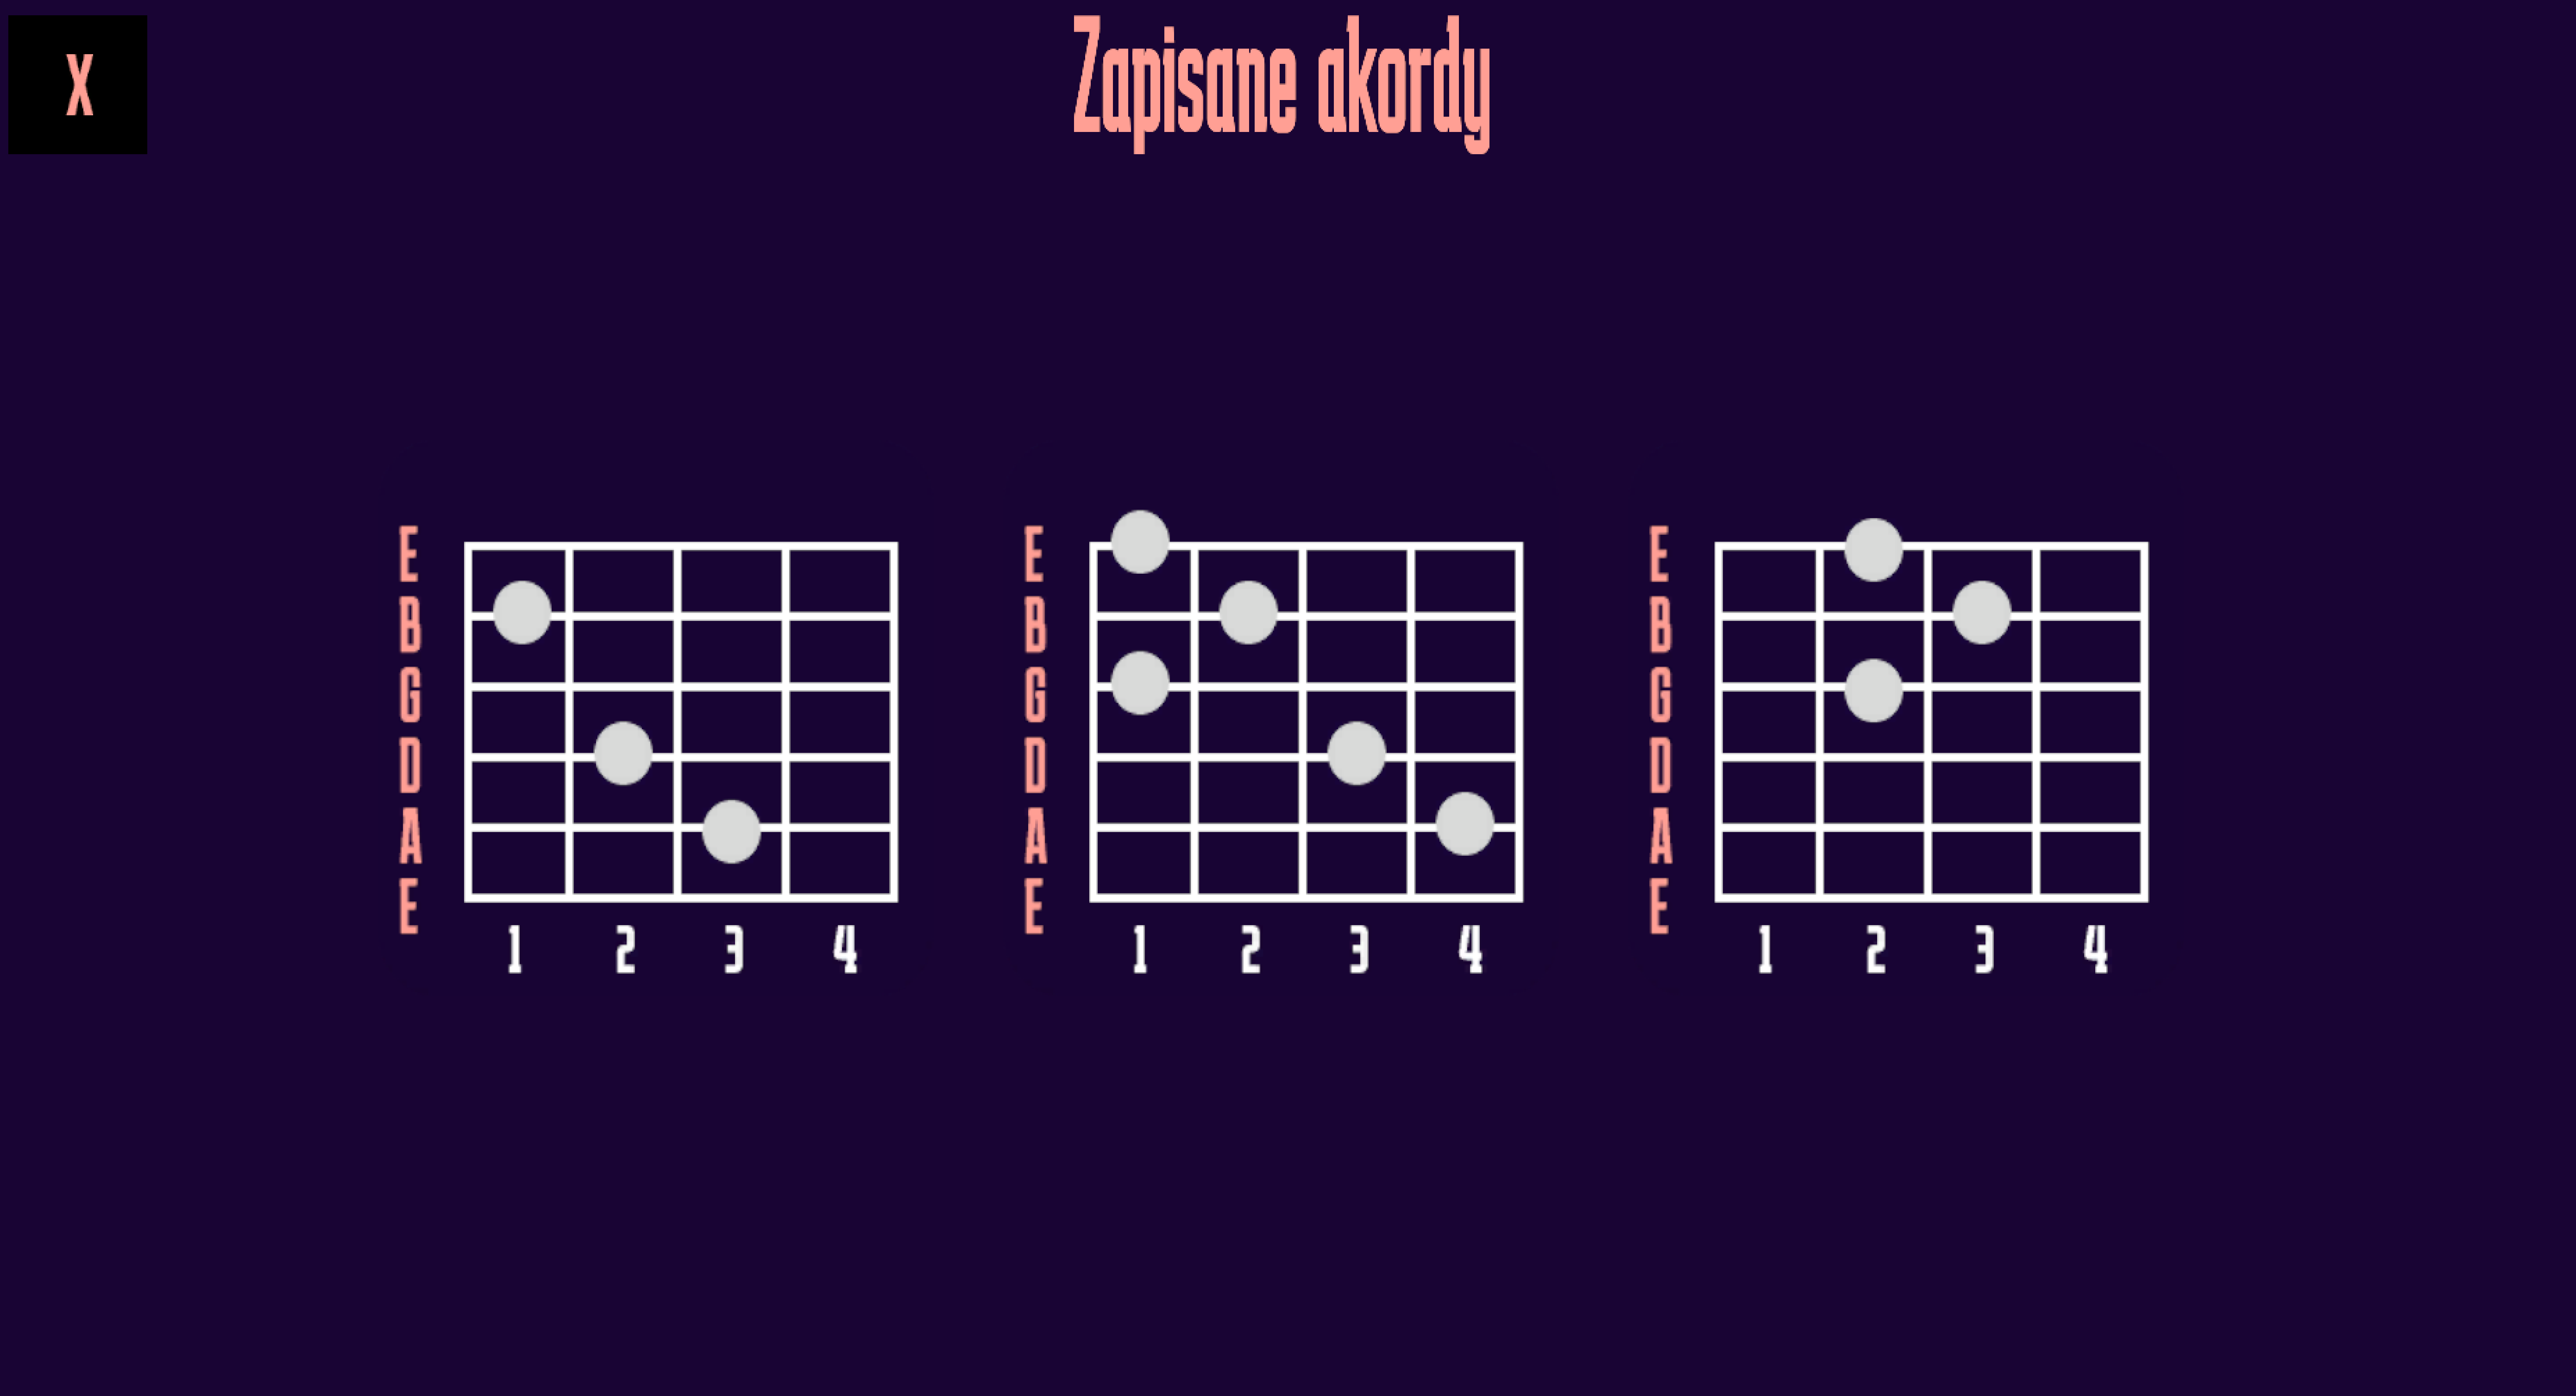
\includegraphics[width=0.6\linewidth]{rysB/Zapisane}}} 
		\end{tabular}
        \caption{Widoki: a) Księga akordów, b) Zapisane akordy}
        \label{fig:Ksiega_Zapisane}
\end{figure}

Użytkownik korzystający z księgi akordów na ekranie zobaczy akord z podaną poniżej jego nazwą. Do zmiany akordu służą 4 przyciski, które można naciskać, aby przeglądać listę dostępnych akordów. Poniżej akordu znajduje się przycisk "Zapisz". Po jego naciśnięciu aktualnie wyświetlany akord zostanie zapisany i będzie dostępny w widoku zapisanych akordów.

\paragraph{Diagram akordów}
Tutaj zobaczyć można wszystkie dostępne w aplikacji akordy (rys.~\ref{fig:DiagramAk}). Użytkownik może przewijać diagram za pomocą dwóch przycisków umieszczonych na dole ekranu. Po naciśnięciu na jeden z akordów użytkownik zostanie przeniesiony do widoku księgi akordów.
\begin{figure}[htb]
	\centering
	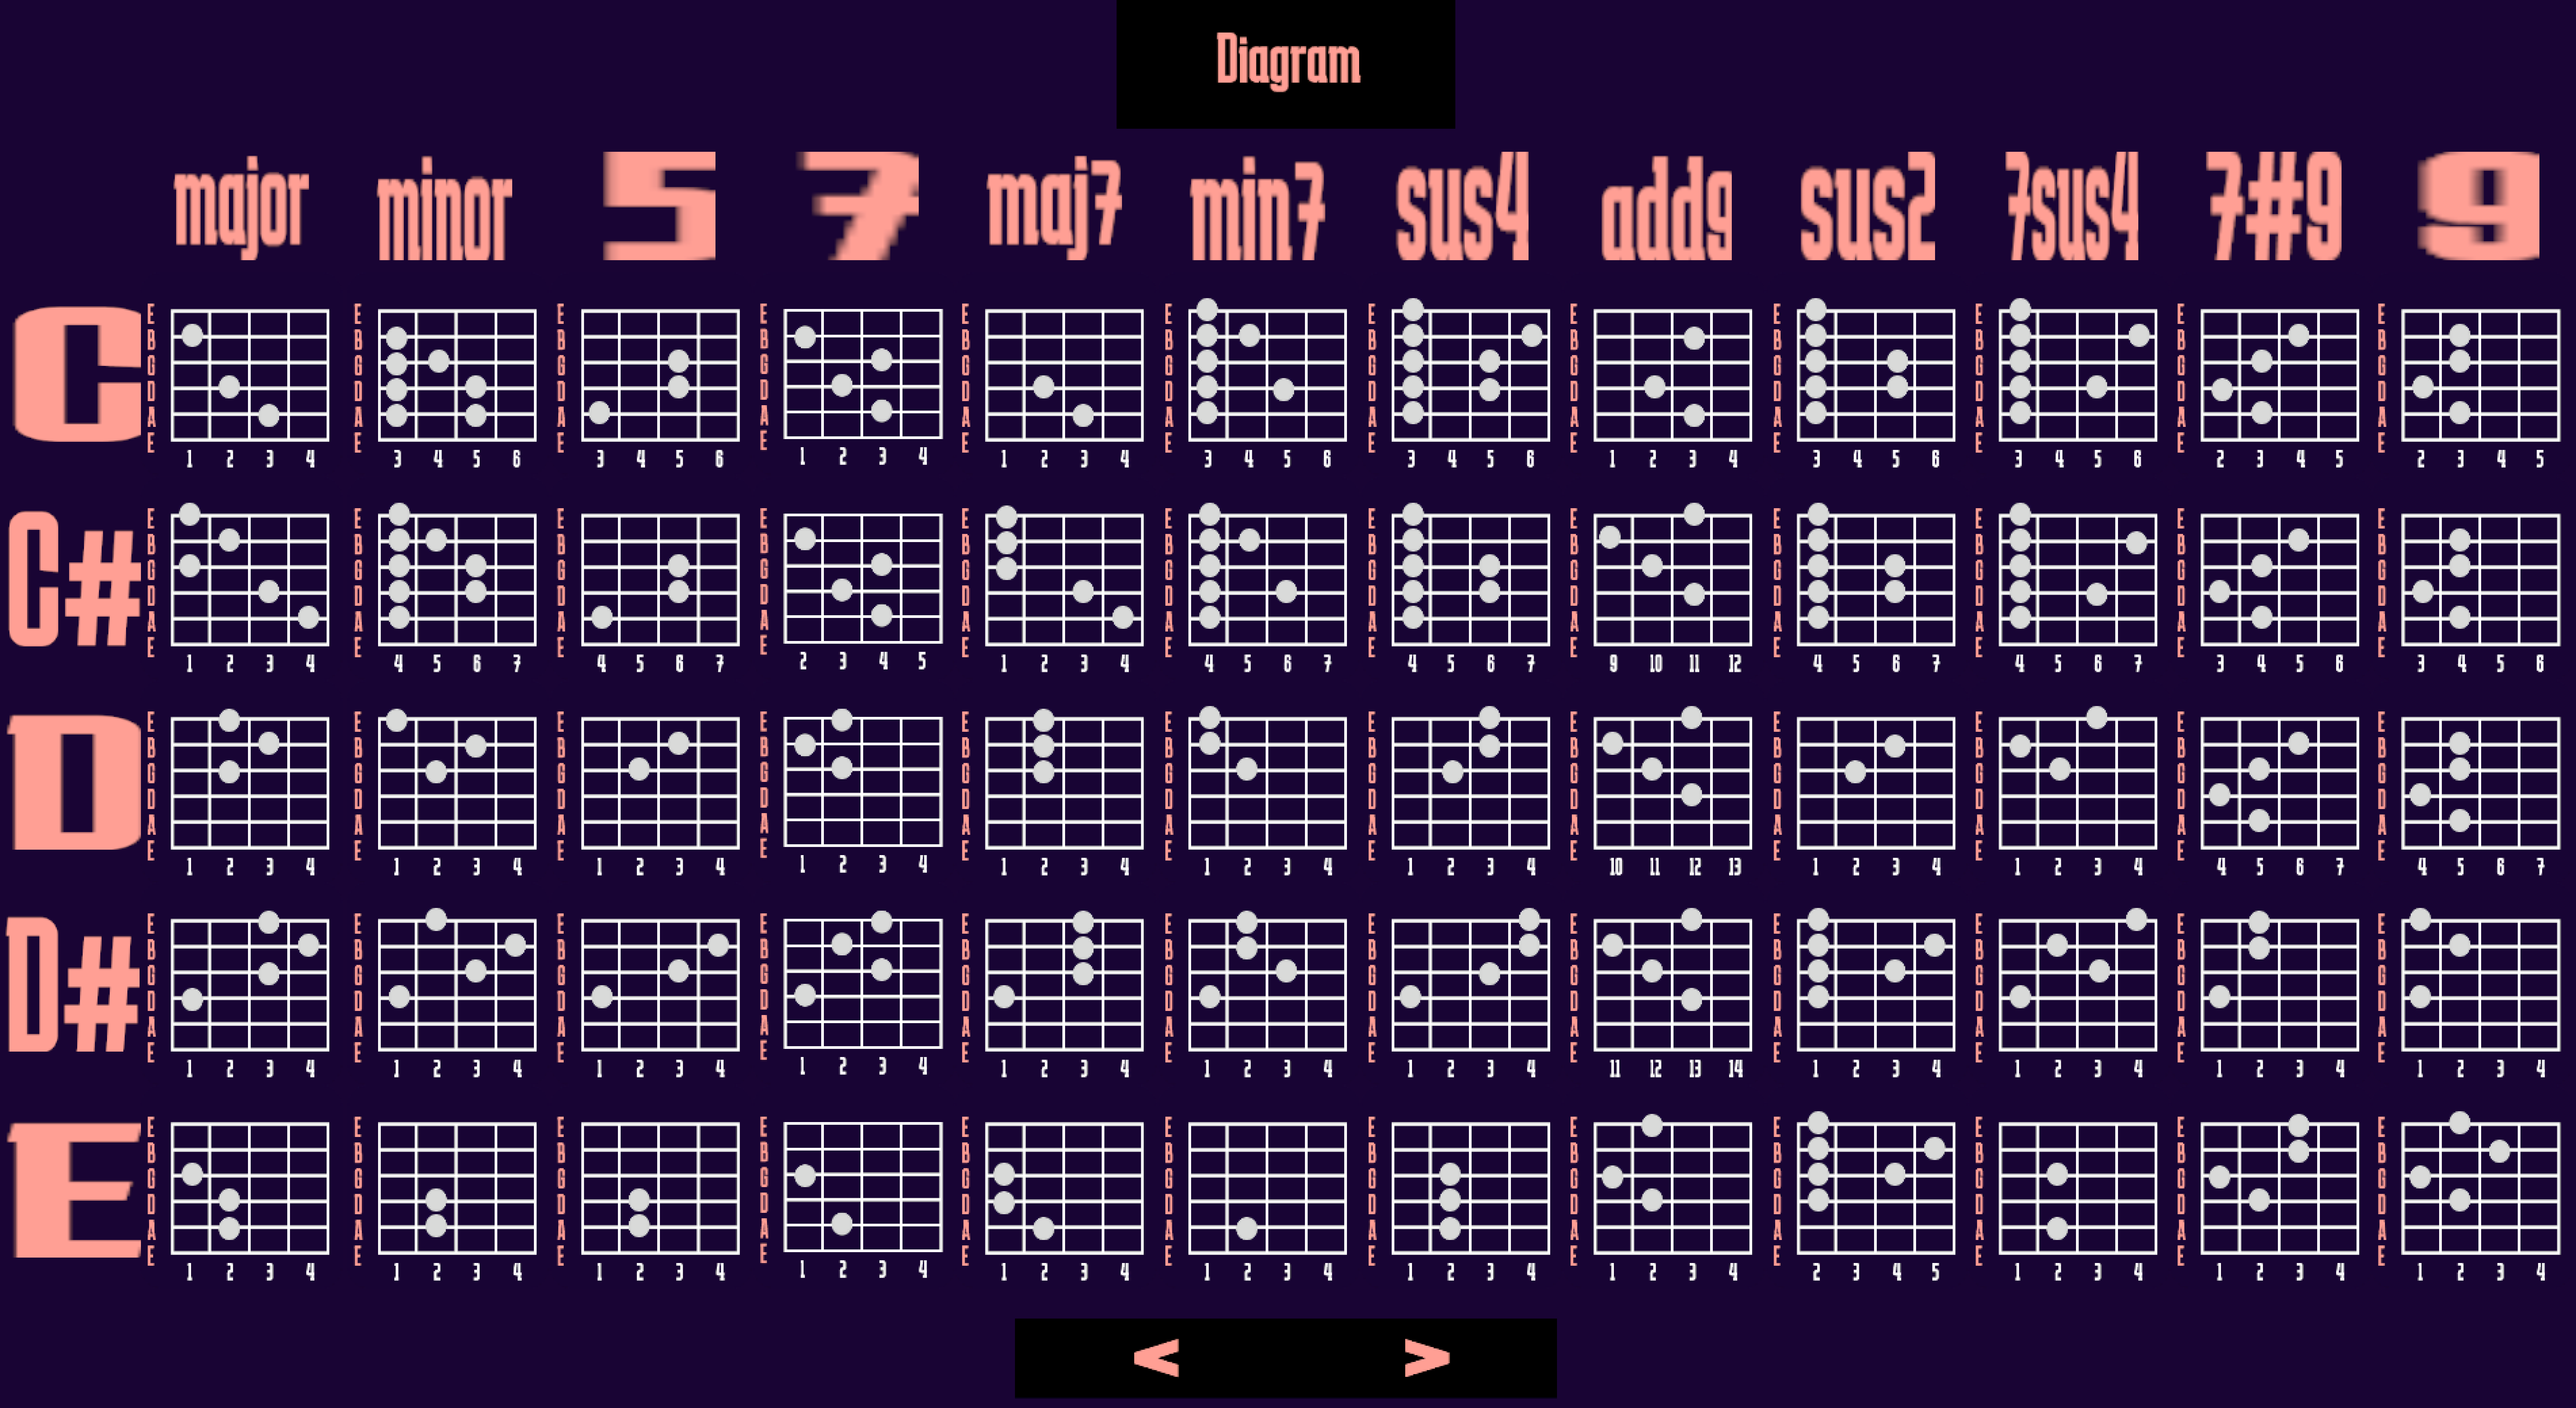
\includegraphics[width=.6\linewidth]{rysB/Diagram}
	\caption{Diagram akordów} \label{fig:DiagramAk}
\end{figure}

\paragraph{Stroik}
Widok stroika (rys.~\ref{fig:Stroik}) pozostał w dużej mierze niezmieniony w stosunku do początkowych założeń. Jedynie strzałki wskazujące poziom nastrojenia zostały zastąpione na znaki "b" oraz "\#", przyjęto te oznaczenia jako ton zaniżony i~zawyżony.
\begin{figure}[htb]
	\centering
	\includegraphics[width=.6\linewidth]{rysB/Stroik}
	\caption{Widok stroika} \label{fig:Stroik}
\end{figure}

Na widoku stroika dostępnych jest 6 przycisków oznaczających nuty gitarowe. Po naciśnięciu jednego z przycisków rozpocznie się faza nagrywania. Wtedy użytkownik powinien wziąć swoją gitarę i uderzyć w docelową strunę. Pośrodku sceny podświetlony zostanie 1 z 3 elementów (patrząc od lewej), oznaczających: zbyt niski ton, dobry ton lub zbyt wysoki ton. Aby skorzystać z narzędzia stroika aplikacja musi mieć dostęp do mikrofonu i~głośników urządzenia, na którym została uruchomiona.


% DONE: tutaj można dodać, że widok zaimplementowany pokrywa się z makietą

\paragraph{Trening słuchu}
Widok treningu słuchu zachował ogólny wygląd zaprojektowany na makiecie. Przyciski odpowiedzi umieszczono wyżej, pod nimi natomiast znalazły się przyciski "GRAJ" i "RESET", odpowiedzialne za uruchomienie i reset treningu.

Scena treningu słuchu (rys.~\ref{fig:TreningS}) wita użytkownika wyborem 4 możliwych tonacji do odbycia treningu. Po wybraniu jednej z 4 możliwych tonacji przed użytkownikiem pojawi się odpowiadająca skala majorowa. Następnie należy nacisnąć przycisk "GRAJ", po czym odgadnąć odegraną nutę za pomocą dostępnych przycisków. W razie chęci zmiany skali należy nacisnąć przycisk "RESET". Po jego naciśnięciu ponownie wyświetlone zostaną 4 możliwe tonacje.

\begin{figure}[htb]
    \centering
    \begin{tabular}{l}
		a) \\
		\vtop{\vskip-2ex\hbox{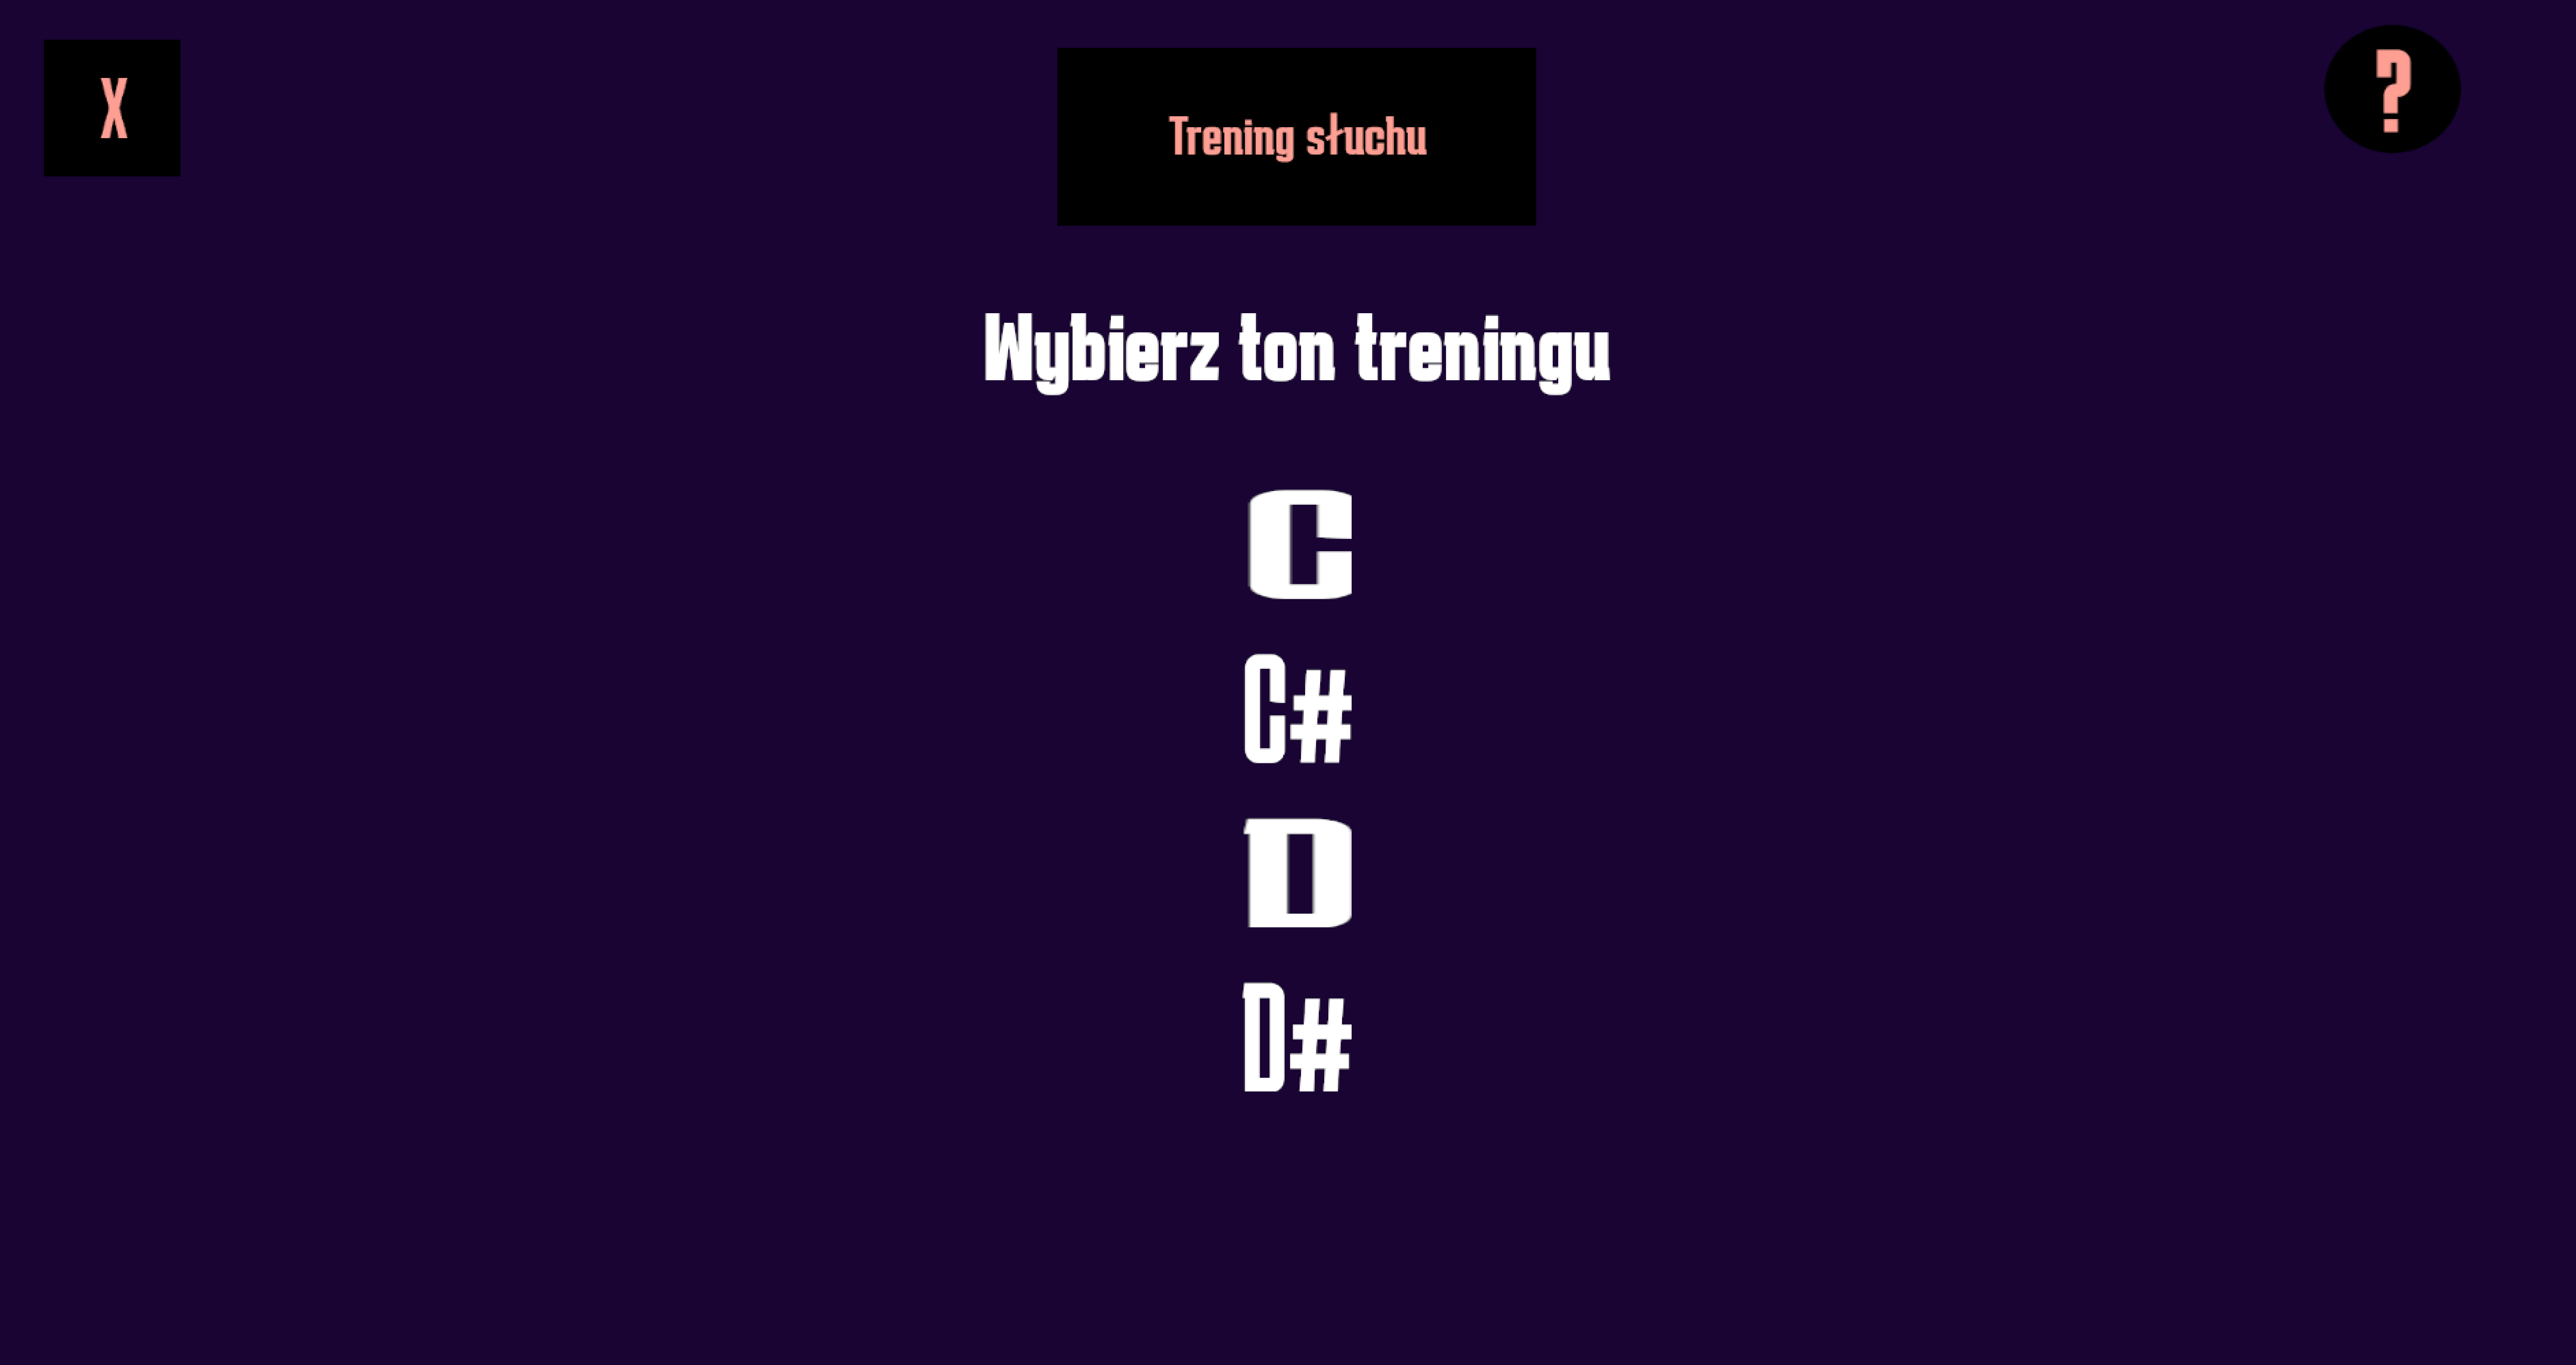
\includegraphics[width=0.6\linewidth]{rysB/Tren1}}} \\
		b) \\
		\vtop{\vskip-2ex\hbox{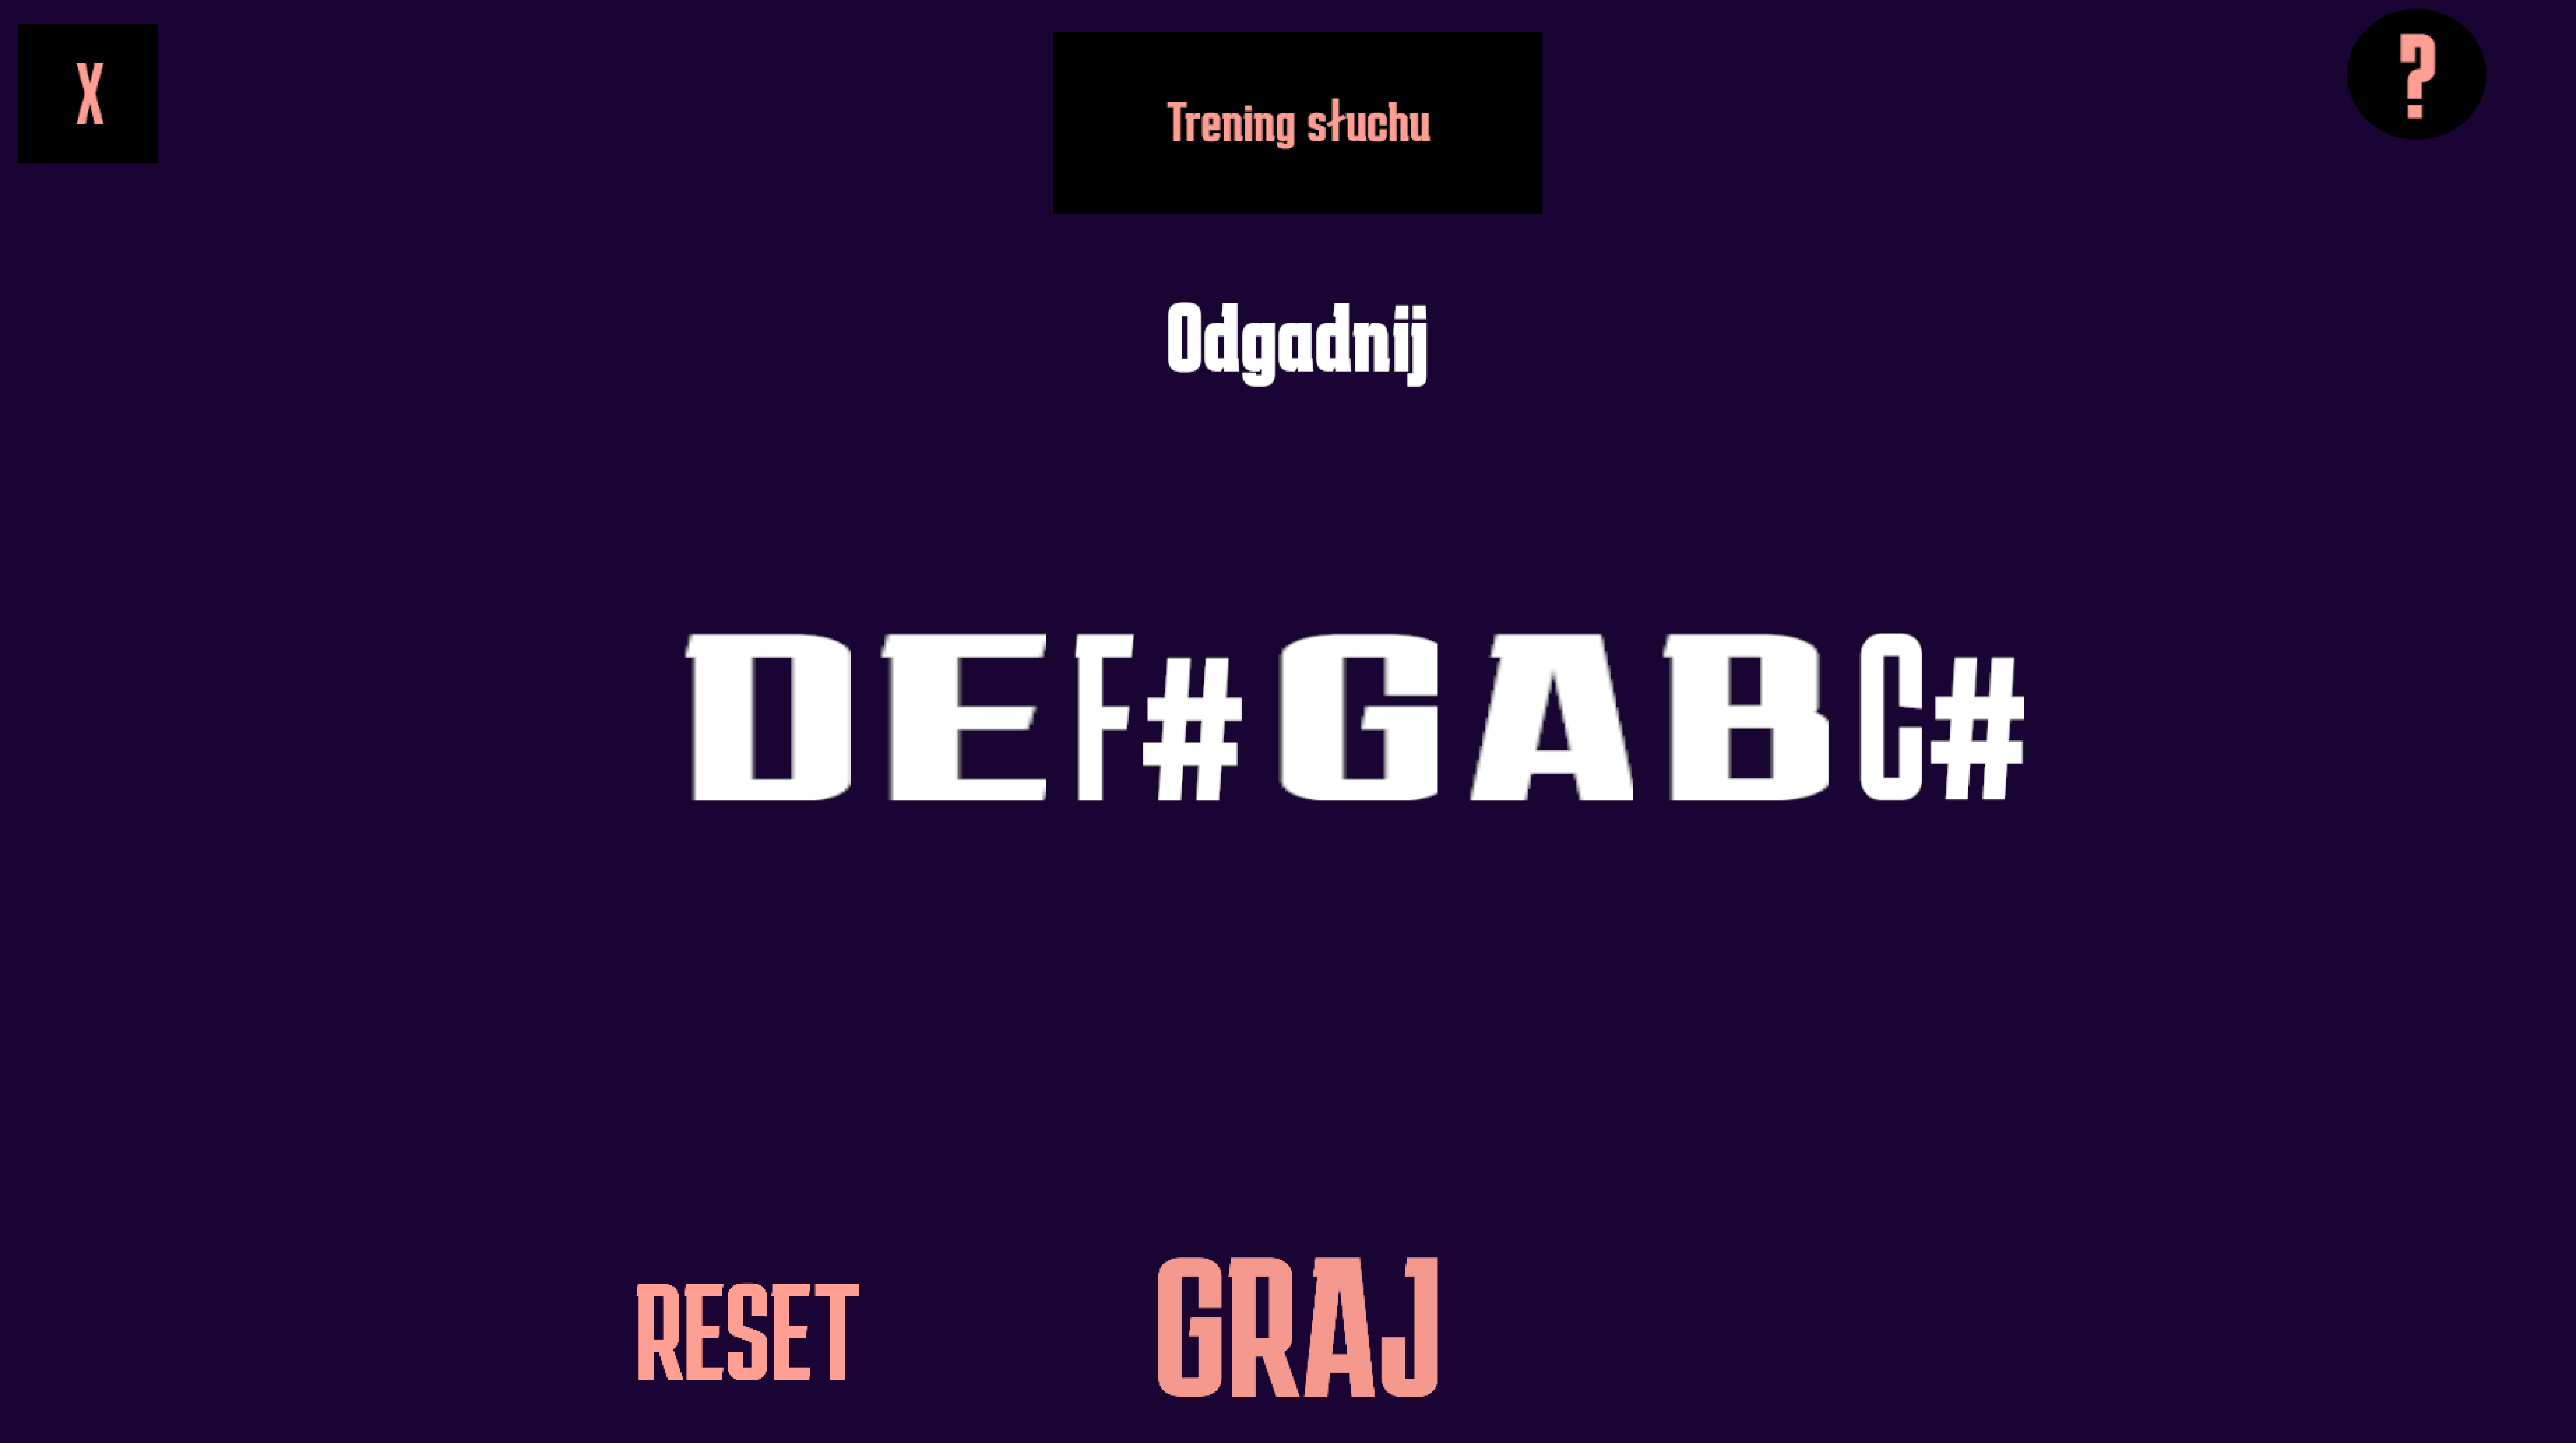
\includegraphics[width=0.6\linewidth]{rysB/Tren2}}} 
		\end{tabular}
    \caption{Widoki treningu muzycznego: a) Widok początkowy, b) Widok po wyborze skali treningowej}
    \label{fig:TreningS}
\end{figure}

% DONE: dodać widok Treningu słuchu. Na makiecie nie było przycisku "GRAJ". Proszę wyjaśnić różnice

\paragraph{Koło kwintowe}
Widok koła kwintowego uległ jedynie rozszerzeniu o wewnętrzne koło nut, przycisk wyjścia i informacji kontekstowej (rys.~\ref{fig:Kolo}).
W obecnej postaci koło to zawiera 12 przycisków zewnętrznych, z którymi użytkownik może wchodzić w~interakcję. Po naciśnięciu jednego z przycisków na zewnętrznym kole, kolorowo zaznaczone zostaną te nuty, które wchodzą w skład skali majorowej, dla której wybrana nuta jest tonem głównym. Ponadto na szaro podświetlą się przyciski symbolizujące akordy pasujące do danej skali.
\begin{figure}[htb]
	\centering
	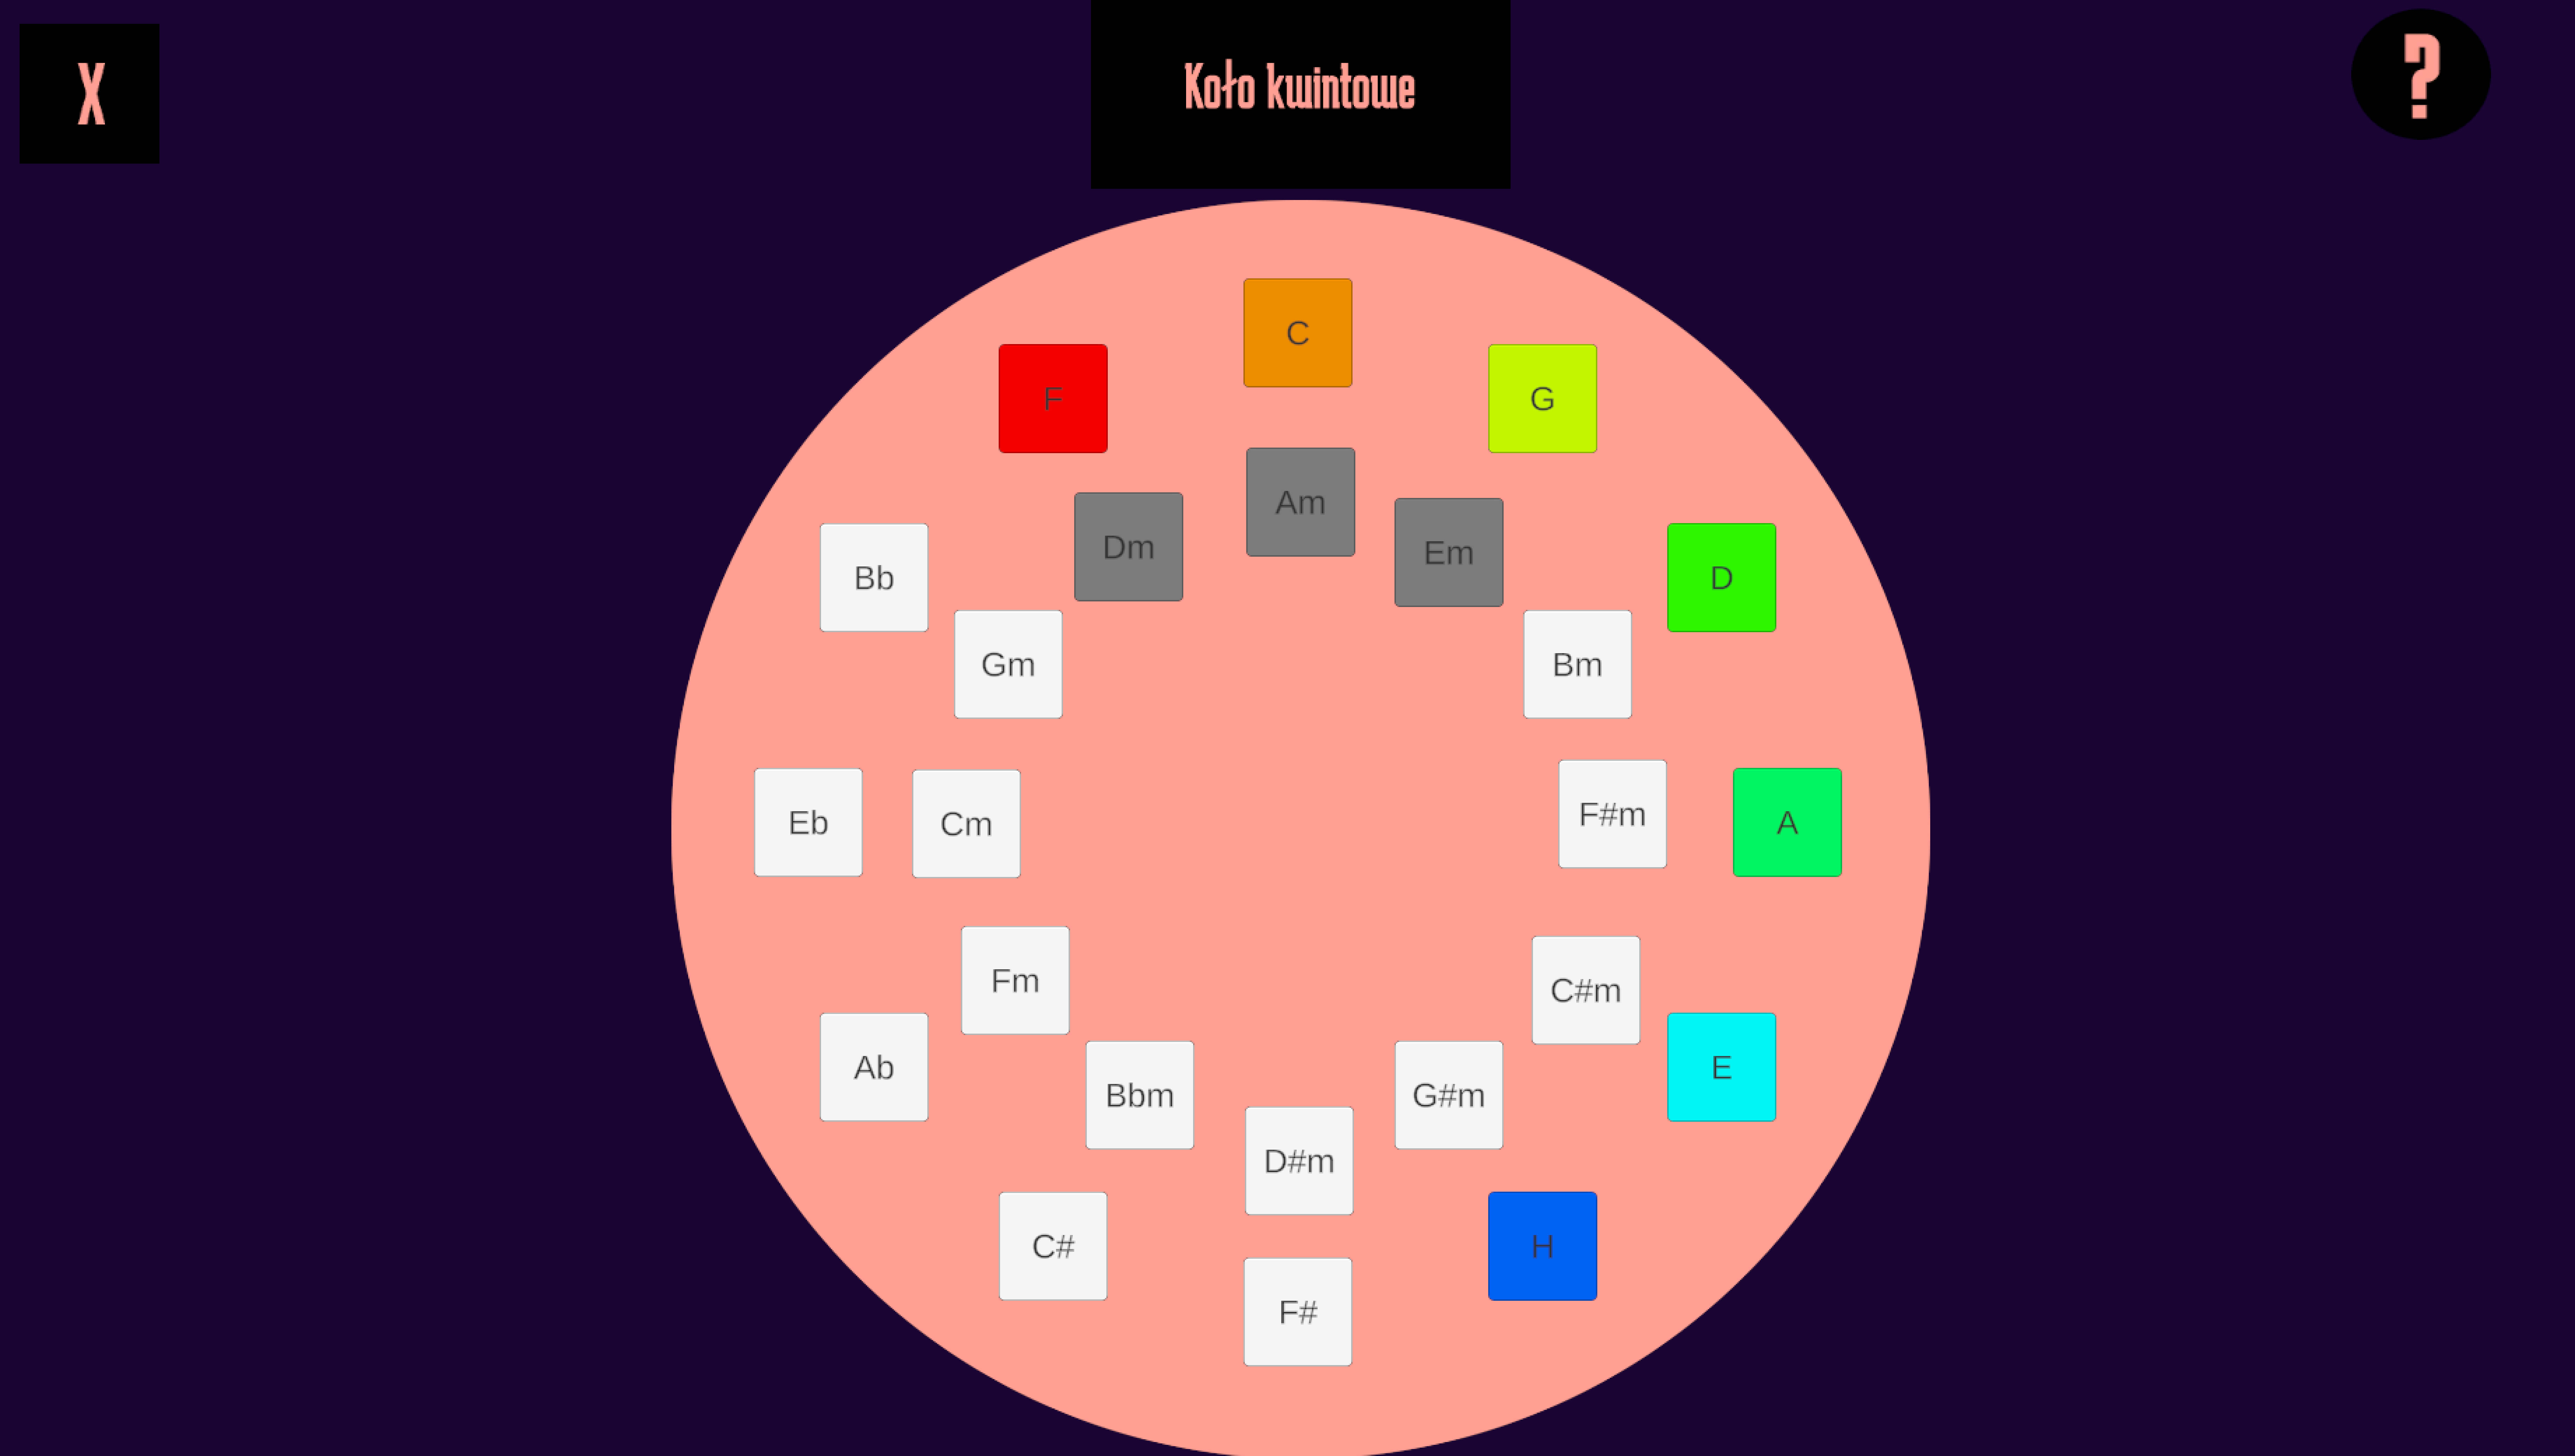
\includegraphics[width=.7\linewidth]{rysB/KoloK}
	\caption{Widok koła kwintowego} \label{fig:Kolo}
\end{figure}

% DONE: dodać widok Koła kwintylowego. Na widoku powinno być widać wyszarzenia (dla przykładowego układu)
